\documentclass{beamer}
 
\usepackage[utf8]{inputenc}
\usepackage{amsmath}
\usepackage{amssymb}
\usepackage{esint}
% \usepackage{physics}

\renewcommand\mathfamilydefault{\rmdefault}
 
 
%Information to be included in the title page:
\title{Electromagnetic Waves Concepts}
\author{Ben Kettle}
\date{16 Jan 2020}
 
\begin{document}
 
\frame{\titlepage}

\begin{frame}{What are Electromagnetic Waves?}
    Recall that changing magnetic fields create electric fields and that changing electric fields create magnetic fields. This fact allows EM waves to propagate. 
    
    \begin{figure}
        \centering
        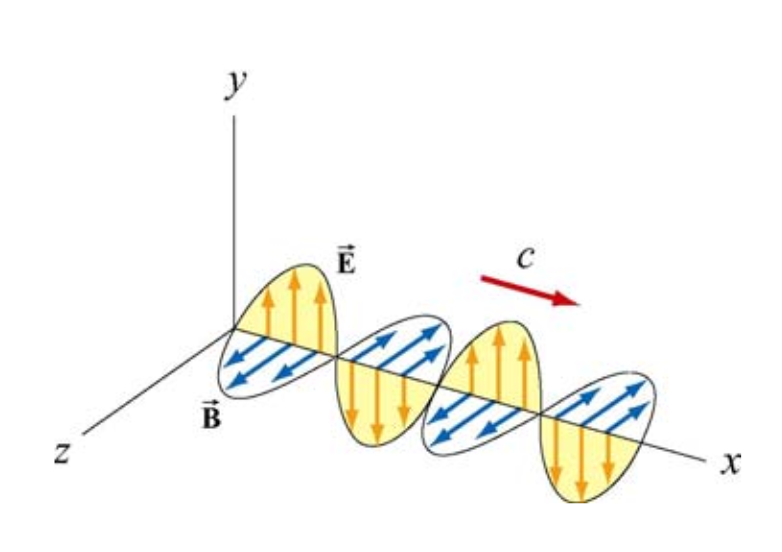
\includegraphics[scale=.4]{emwave.png}
        \caption{An electromagnetic wave.}
        \label{fig:emwave}
    \end{figure}
\end{frame}

\begin{frame}{Maxwell's Equations}
    \begin{columns}
    \begin{column}{0.5\textwidth}
        \begin{center}
            Gauss's Law for $\vec{\mathbf{E}}$
        \end{center}
       \[ \oiint_S \vec{\mathbf{E}}\cdot d\vec{\mathbf{A}} = \frac{Q}{\varepsilon_0} \]
       Electric  flux  through  a  closed  surfaceis proportional to the charged enclosed
       \end{column}
       \begin{column}{0.5\textwidth}
        \begin{center}
            Faraday's Law
        \end{center}
        \[ \oint \vec{\mathbf{E}}\cdot d\vec{\mathbf{s}} = -\frac{d\Phi_B}{dt}\]
        Changing  magnetic  flux  produces  an  electric field 
    \end{column}
    \end{columns}
    
    \begin{columns}
    \begin{column}{0.5\textwidth}
        \begin{center}
            Gauss's Law for $\vec{\mathbf{B}}$
        \end{center}
       \[ \oiint_S \vec{\mathbf{B}}\cdot d\vec{\mathbf{A}} = 0 \]
       The   total   magnetic   flux   through   a closed surface is zero 
       \end{column}
       \begin{column}{0.5\textwidth}
        \begin{center}
            Ampere-Maxwell Law
        \end{center}
        \[ \oint \vec{\mathbf{B}}\cdot d\vec{\mathbf{s}} = \mu_0 I + \mu_0\varepsilon_0\frac{d\Phi_E}{dt}\]
        Electric  current  and  changing  electric  flux produces a magnetic field
    \end{column}
    \end{columns}
\end{frame}

\begin{frame}{Maxwell's Equations in Empty Space}
    When we assume $Q=0$ and $I=0$, as is the case for travelling electromagnetic waves, these get a bit simpler:
    \begin{columns}
    \begin{column}{0.5\textwidth}
        \begin{center}
            Gauss's Law for $\vec{\mathbf{E}}$
        \end{center}
       \[ \oiint_S \vec{\mathbf{E}}\cdot d\vec{\mathbf{A}} = 0 \]
        \begin{center}
            Faraday's Law
        \end{center}
        \[ \oint \vec{\mathbf{E}}\cdot d\vec{\mathbf{s}} = -\frac{d\Phi_B}{dt}\]
    \end{column}
    
    \begin{column}{0.5\textwidth}
        \begin{center}
            Gauss's Law for $\vec{\mathbf{B}}$
        \end{center}
       \[ \oiint_S \vec{\mathbf{B}}\cdot d\vec{\mathbf{A}} = 0 \]
        \begin{center}
            Ampere-Maxwell Law
        \end{center}
        \[ \oint \vec{\mathbf{B}}\cdot d\vec{\mathbf{s}} = \mu_0\varepsilon_0\frac{d\Phi_E}{dt}\]
    \end{column}
    \end{columns}
\end{frame}

\begin{frame}{EM Wave Basics}
    A key fact for electromagnetic waves is that they are \alert{transverse}---both the $\vec{E}$ and $\vec{B}$ fields are perpendicular to the direction of propagation. The fields are also perpendicular to each other, so where $\vec{\mathbf{p}}$ is the direction of propagation:
    \[ \vec{\mathbf{E}} \times \vec{\mathbf{B}} = \vec{\mathbf{p}} \]
    
\end{frame}

\begin{frame}{The Wave Equation for EM waves}
    Our goal is to find the \alert{wave equation} for the EM wave---something of the form:
    \[ \left(\frac{\partial^2}{\partial x^2}-\frac{1}{v^2}\frac{\partial^2}{\partial t^2}\right)\psi(x,t)=0 \]
    
    Where $\psi(x,t)$ is the wave function itself and $v$ is the wave velocity. To do this, we will apply Faraday's Equation and the Ampere-Maxwell law to an electromagnetic wave. 
    
\end{frame}

\begin{frame}{The Wave Equation for EM waves}
    \begin{columns}
    \begin{column}{.5\textwidth}
    Setting our coordinate system such that the $\vec{E}$ field is in the $xy$ plane and the $\vec{B}$ field is in the $xz$ plane, the wave equation for an electromagnetic wave can be found using multivariable calcalculus. \vspace{2mm}
    
    Using the Faraday Equation, we can integrate over a loop in the $xy$ plane to find:
    \[ \frac{\partial E_y}{\partial x} = -\frac{\partial B_z}{\partial t} \]
    \end{column}
    \begin{column}{.5\textwidth}
        \begin{figure}
            \centering
            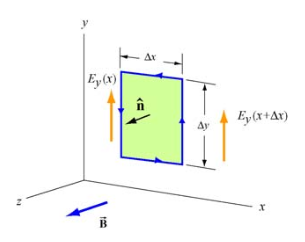
\includegraphics[scale=.8]{efieldint.png}
            \caption{Applying Faraday's Law to a loop in the $xy$ plane.}
            \label{fig:my_label}
        \end{figure}
    \end{column}
    \end{columns}
\end{frame}

\begin{frame}{The Wave Equation for EM waves}
    Then, following the same steps with Ampere-Maxwell and a loop in the $xz$ plane, we reach:
    \[ - \frac{\partial B_z}{\partial x} = \mu_0\varepsilon_0\frac{\partial E_z}{\partial t}\]
    \begin{figure}
        \centering
        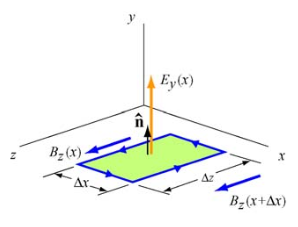
\includegraphics[scale=.9]{bfieldint.png}
        \caption{Applying Ampere-Maxwell to a loop in the $xz$ plane.}
        \label{fig:my_label}
    \end{figure}
\end{frame}

\begin{frame}{Velocity of an EM Wave}
    The equation describing any wave is given in a general form of:

    \[ \left(\frac{\partial^2}{\partial x^2}-\frac{1}{v^2}\frac{\partial^2}{\partial t^2}\right)\psi(x,t)=0 \]
    Where $\psi(x,t)$ is the wave function itself and $v$ is the wave velocity. More manipulation of the two equations from the last sides yields us something in a similar format:
    \[  \left(\frac{\partial^2}{\partial x^2}-\mu_0\varepsilon_0\frac{\partial^2}{\partial t^2}\right)\left\{ \begin{array}{c} E(x,t) \\ B(x,t) \end{array} \right\}=0 \]

    We can then clearly find the velocity of an electromagnetic wave:
    \[ \frac{1}{v^2} = \mu_0\varepsilon_0 \longrightarrow v = \frac{1}{\sqrt{\mu_0\varepsilon_0}}\]
\end{frame}

\begin{frame}{Proving that light is an EM wave}
    We can use this fact to show that light is an example of an electromagnetic wave.
    
    \[ v=\frac{1}{\sqrt{\mu_{0} \varepsilon_{0}}}=\frac{1}{\sqrt{\left(4 \pi \times 10^{-7} T \cdot m/A\right)\left(8.85 \times 10^{-12} C^{2} / N \cdot m^{2}\right)}} \] 
    \[ v =2.997 \times 10^{8} m/s=c \]
\end{frame}

\begin{frame}{More EM Wave Properties}
    Had we done the full derivation of the above fact, we would also be able to show that:
    \[ \frac{E}{B} = c \] 
    This means that in an electromagnetic wave, the $\vec{E}$ field is much larger than the $\vec{B}$ field.
\end{frame}

\begin{frame}{Summary: The Important Slide}
    That was probably confusing. So to summarize what we know:
    \begin{itemize}
	\item The wave is transverse because $\vec{E}$ and $\vec{B}$ are perpendicular to the direction of propagation $\vec{p}$, which is given by $\vec{p} = \vec{E} \times \vec{B}$.
	\item The $E$ and $B$ fields are perpendicular to each other, meaning $\vec{E} \cdot \vec{B} = 0$.
	\item $\frac{E}{B} = \frac{E_0}{B_0} = c$
	\item The wave's speed of propagation equals $\frac{1}{\sqrt{\mu_0\epsilon_0}}$
	\item The superposition principle applies to the waves---two overlapping waves can be added to give the resulting wave.
    \end{itemize}
\end{frame}

\begin{frame}{Electromagnetic Wave Creation}
    Generally, EM waves are created by charges moving in space. In practice, most EM waves are created using an antenna by applying an AC current to the center. This causes charges to oscillate between the two ends of the antenna. \vspace{2mm}

    However, the fields created close to the antenna (in the \alert{near field}) do not behave like EM radiation. It's only far away from the transmitter (in the \alert{far field}), where most of these fields have returned their energy to the transmitter, that we see EM radiation as we expect. 
    
    \begin{figure}
        \centering
        
\includegraphics[scale=.13]{nearfar.png}
        \label{fig:nearfar}
    \end{figure}
    
\end{frame}

\begin{frame}{Antenna}
    Electromagnetic waves are often created by an antenna:
    \begin{figure}
        \centering
        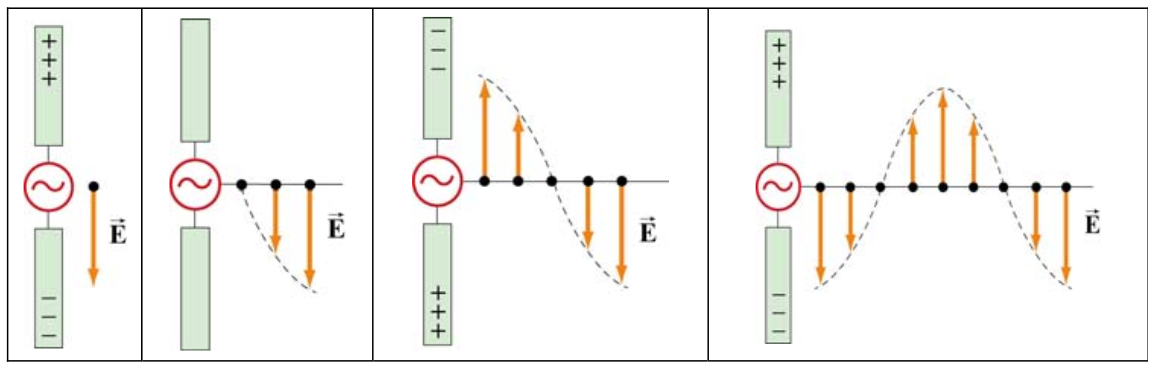
\includegraphics[scale=.4]{antenna.png}
        \caption{An antenna creating an EM wave}
        \label{fig:antenna}
    \end{figure}
\end{frame}

\begin{frame}{EM Spectrum}
    There are many other types of EM waves, defined by their frequencies:

    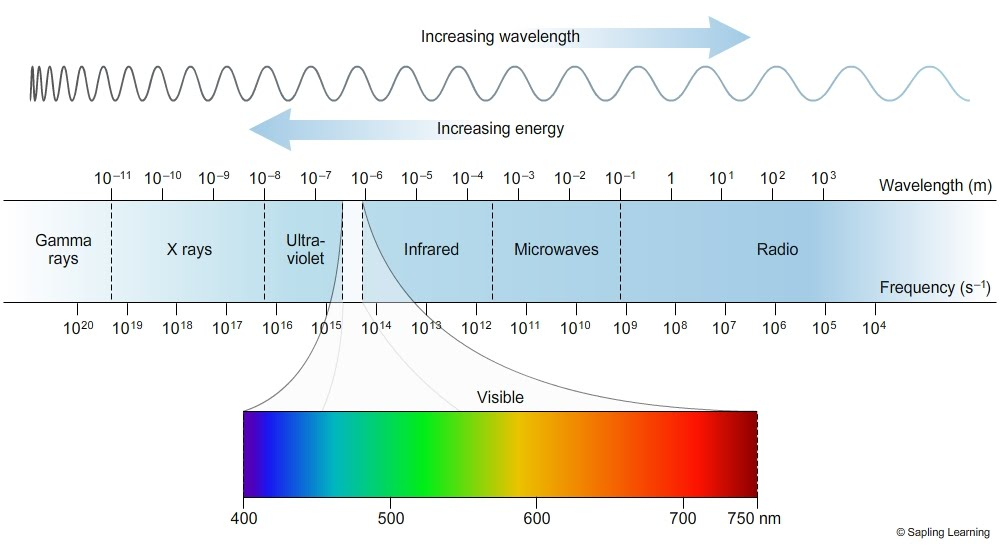
\includegraphics[scale=.3]{emspectrum.jpg}
    
\end{frame}

\begin{frame}{Radio Waves}
	\begin{center}
	\begin{tabular}{c c}
		Frequency & Wavelength \\
		$30 Hz - 300 GHz$ & $1 mm - 10,000 km$ \\	
	\end{tabular}
	\end{center}
	Clearly, radio waves cover a large part of the spectrum. Within radio waves, different wavelengths have different characteristics:
	\begin{itemize}
		\item Long wavelengths---such as AM radio---can diffract around obstacles such as mountains. These waves are also able to follow the contour of the earth instead of travelling into space. 
		\item Shorter wavelengths are unable to follow the earth and don't diffract as well, but are able to reflect off of the atmosphere, allowing them to travel over the horizon.
		\item Very short wavelengths ($\geq 30 MHz$) in this spectrum lose the ability to reflect off the atmosphere, and become limited to \alert{line of sight} (about 64km).  
	\end{itemize}
\end{frame}

\begin{frame}{Low Frequency Waves}
	\begin{center}	
	\begin{tabular}{ccc}
		name & frequency & uses \\ \hline
		Low Frequency & 30 kHz & Time Signals  \\
		Very Low Frequency & 3 kHz & \\
		Ultra Low Frequency & 300 Hz & Earth-Mode Communication\\
		Super Low Frequency & 30 Hz & Submarine Communication \\
		Extremely Low Frequency & 3 Hz & Submarine Communication
	\end{tabular} 
	\end{center}
	
\begin{columns}
	\begin{column}{.7\textwidth}
	In the very low end of the EM wave spectrum, a subset of radio waves, we have the amusingly named low frequency radio waves. In general, the lower the frequency, the farther the wave travels in the presence of obstacles. However, shorter wavelengths also limit the data transmission rate heavily and require huge antennas to transmit.
	\end{column}
	\begin{column}{.3\textwidth}
	\begin{figure}
	    \centering
	    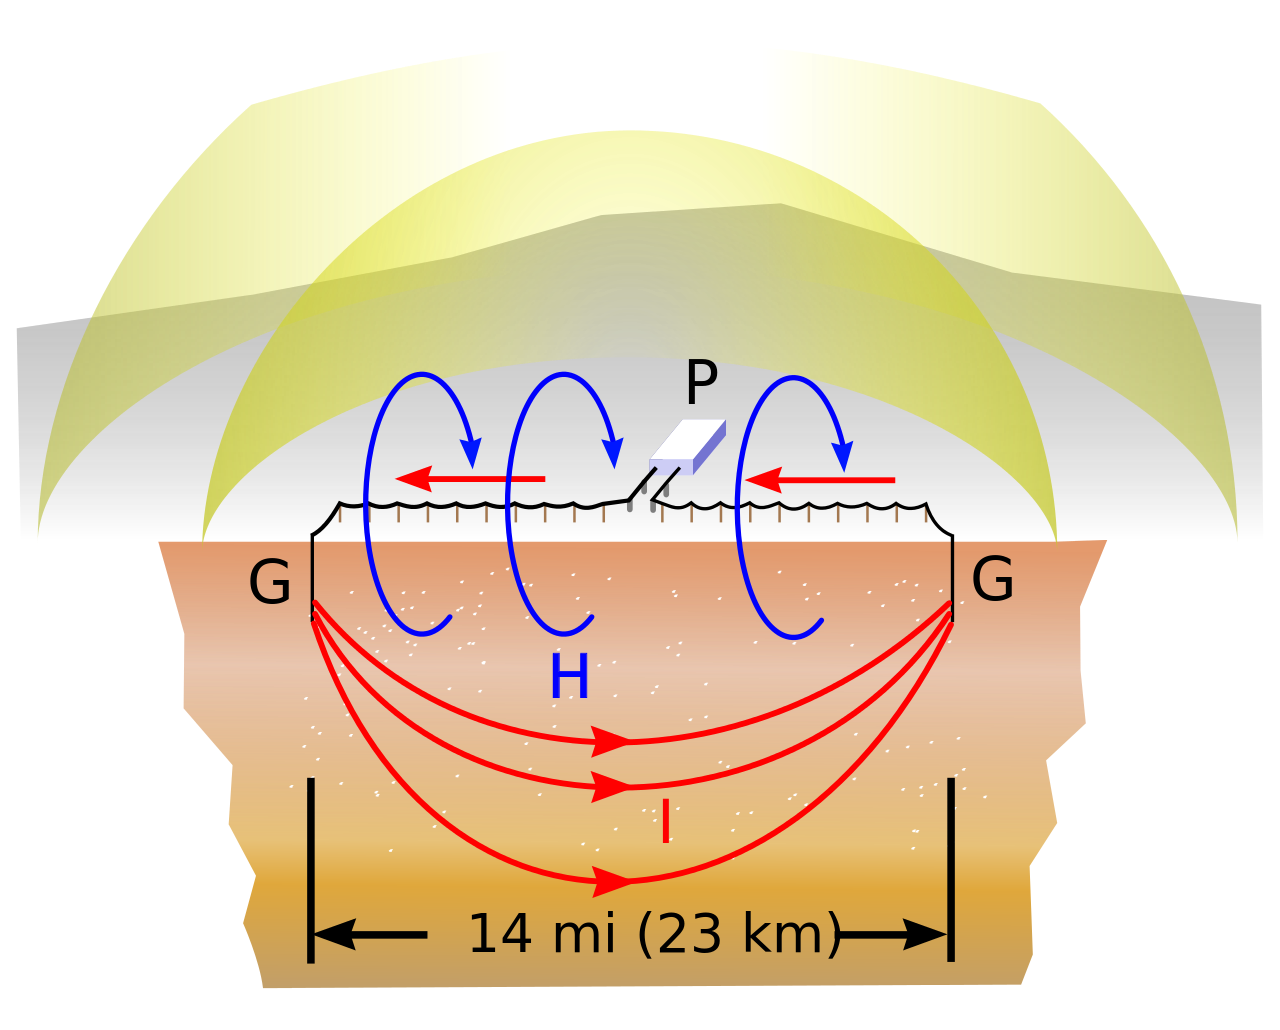
\includegraphics[scale=.08]{elf_antenna.png}
	    \label{fig:elf_antenna}
	\end{figure}
	\end{column}
\end{columns}
\end{frame}

\begin{frame}{AM/FM Radio}
    \begin{columns}
	\begin{column}{.6\textwidth}
	Perhaps the most obvious use of radio waves is in radios, where they are used to transmit audio. In AM, this happens through modulating the amplitude of the wave, while in FM this happens through modulating the frequency. \vspace{5mm}
	
	These AM waves travel much farther, but are very susceptible to noise. FM is limited in distance but provides better quality audio.
	\end{column}
	\begin{column}{.4\textwidth}
	\begin{figure}
	    \centering
	    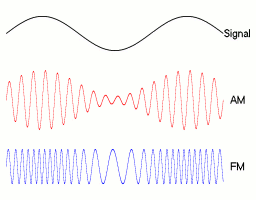
\includegraphics[scale=.4]{amfm.png}
	    \caption{A signal and the corresponding AM/FM waves.}
	    \label{fig:amfm}
	\end{figure}
	\end{column}
\end{columns}
\end{frame}

\begin{frame}{Radio: Receiving EM Waves}
    Receiving waves, like transmitting them, usually uses an antenna. In this case, the antenna will generate an AC current in whatever it is connected to. Receiving EM waves usually involves the use of a tuned circuit, or \alert{band-pass filter}. In essence, this is an LC circuit driven by the antenna input.
    \begin{itemize}
	    
	    \item What characteristic of an LC circuit might be useful in creating a circuit that has meaningful output at only a certain frequency? \visible<2->{\alert{An LC circuit will achieve its maximum output only when in resonance. For this to happen, the input frequency must match the circuit's resonance frequency $\omega_0$. When this condition is not met, the circuit will not output meaninful current to the amplifier and speaker. }}
    \end{itemize}
\end{frame}

% \begin{frame}{Radio: LC Circuit Practice}
% 	\begin{columns}
% 	\begin{column}{.6\textwidth}
% 	\begin{itemize}
% 	\item For the LC circuit to the right with $L = 10 H$ and $C= 40 F$, what is the resonance frequency? Recall that we want to minimize impedance. \visible<3->{\alert{gotta write this solution}}
% 	\end{itemize}
% 	\end{column}
% 	\begin{column}{.4\textwidth}
% 		
\includegraphics[scale=.2]{lc.png}
% 	\end{column}
% 	\end{columns}
% \end{frame}

\begin{frame}{Application in a Radio}
	\begin{columns}
	\begin{column}{.6\textwidth}
    Radios now have many more similar circuits to eliminate noise and amplify the signal, but the basic functionality of "tuning a radio" depends on this behavior.
    \begin{itemize} \item How could we allow a user to select what frequency they would like to filter for? \visible<2->{\alert{Modifying either the capacitance or inductance would work. It turns out it's easy to make a variable capacitor, though, so that is how it's typically done.}} \end{itemize}
	\end{column}	
	\begin{column}{.4\textwidth}
	    \visible<2->{\begin{figure}
	    \centering
	    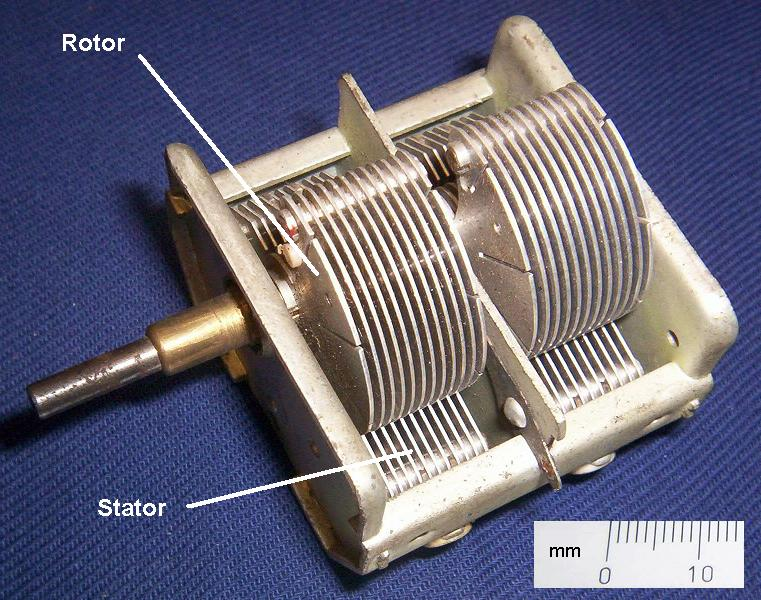
\includegraphics[scale=.5]{rotarycap1.jpg}
	    \vspace{1mm}
        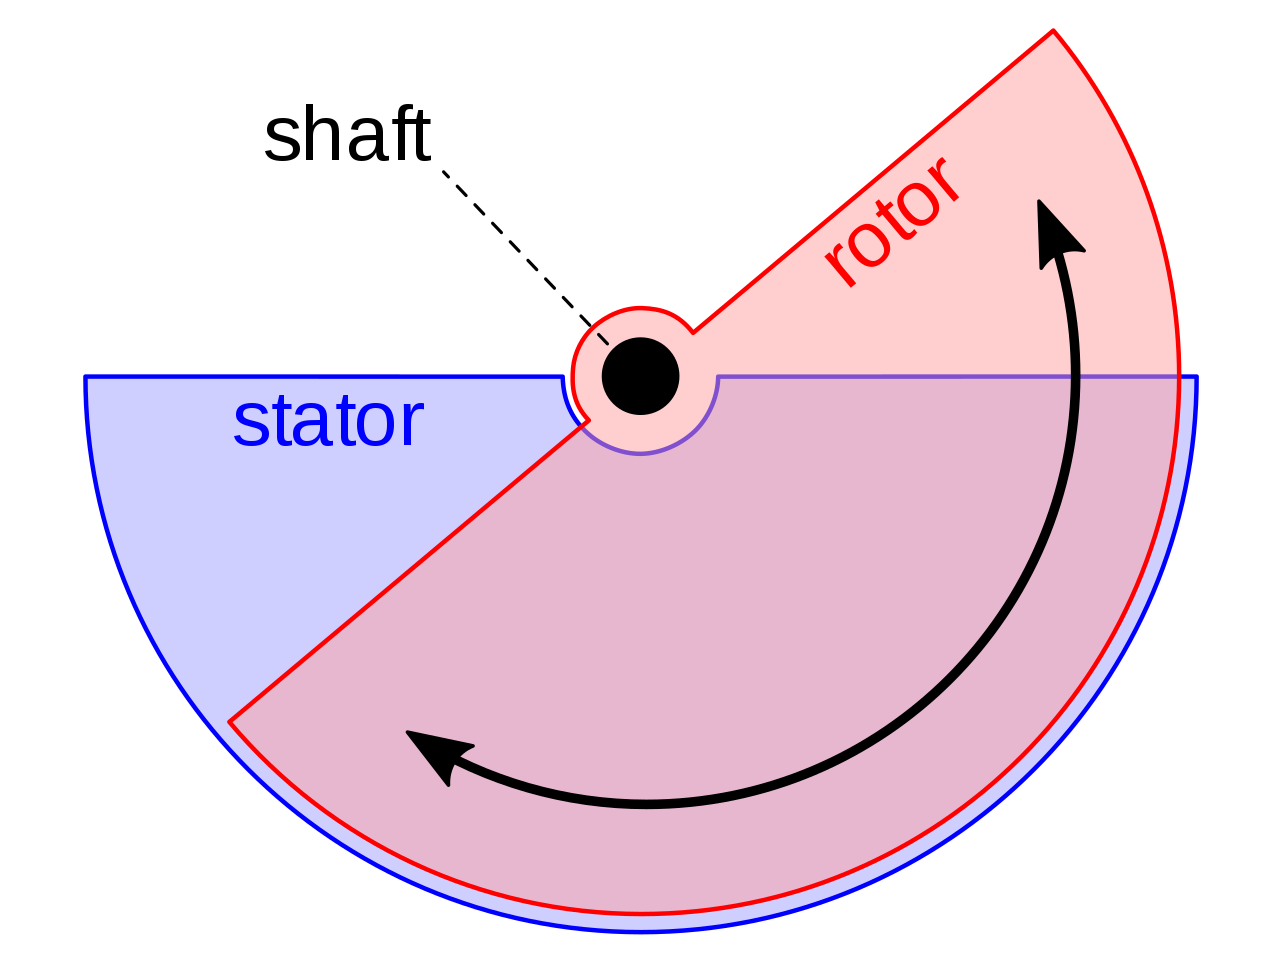
\includegraphics[scale=.07]{rotarycap2.png} 
	    \caption{The operation of a variable capacitor}
	    \label{fig:rotarycap}
	    \end{figure}}
	\end{column}
	\end{columns}
\end{frame}

\begin{frame}{Microwaves}
	Microwaves (300MHz - 300GHz) are a higher-frequency subset of radio waves. They are generally limited by the 64km line-of-sight limit, as they do not diffract around hills or follow the earth's surface. As usual, this range decreases as frequency increaes, in this case because short-wavelength waves are absorbed by the atmosphere.
\end{frame}

\begin{frame}{Microwave Creation}
	\begin{columns}
	\begin{column}{.6\textwidth}
    Microwaves are often generated using some form of vacuum tube, taking advantage of the interaction of moving electrons with a magnetic field to generate microwaves. \vspace{2mm}
    
    One of the most common examples, a microwave oven, uses a magnetron. A magnetron is a form of vacuum tube that includes chambers that microwaves resonate in. Because charges travel on the surface of the conductor in AC circuits, the structure causes the magnetron to act like an LC circuit.
    
	\end{column}	
	\begin{column}{.4\textwidth}
	    \begin{figure}
	    \centering
	    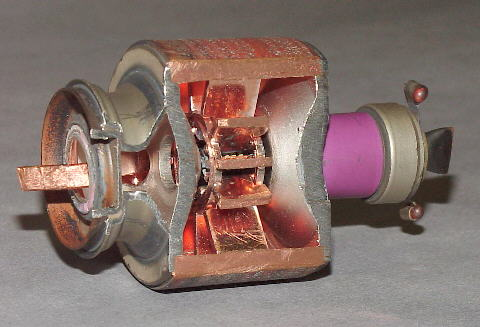
\includegraphics[scale=.3]{magnetron1.jpg}
	    \vspace{1mm}
        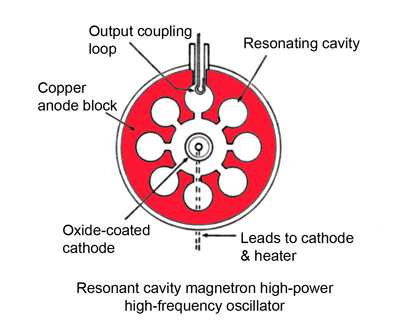
\includegraphics[scale=1]{magnetron2.png} 
	    \caption{A microwave oven magnetron.}
	    \label{fig:rotarycap}
	    \end{figure}
	\end{column}
	\end{columns}
\end{frame}

\begin{frame}{Microwave Ovens}
    When microwaves pass through food, they can create heating. This happens because many molecules (water and fat, for example) are electric dipoles, and rotate continuously to align with the changing $\vec{E}$ field that the EM wave provides. Most microwave ovens operate at $2.45$ GHz, but there is a range of frequencies that work.\vspace{5mm}
    
    Microwaves are also used for WiFi, for cell phone networks, for GPS, and in many other applications. 
\end{frame}

\begin{frame}{Airport Scanning}
\begin{columns}
    \begin{column}{.5\textwidth}
        Microwaves are also used for security scanning at airports in "millimeter wave" scanning machines. As you can guess, these take advantage of microwaves with a wavelength of $1mm$. They operate by transmitting microwaves from two antennas and measuring the way the waves reflect. Skin and other objects will reflect the waves, but clothing won't.
    \end{column}
    \begin{column}{.5\textwidth}
    \begin{figure}
        \centering
        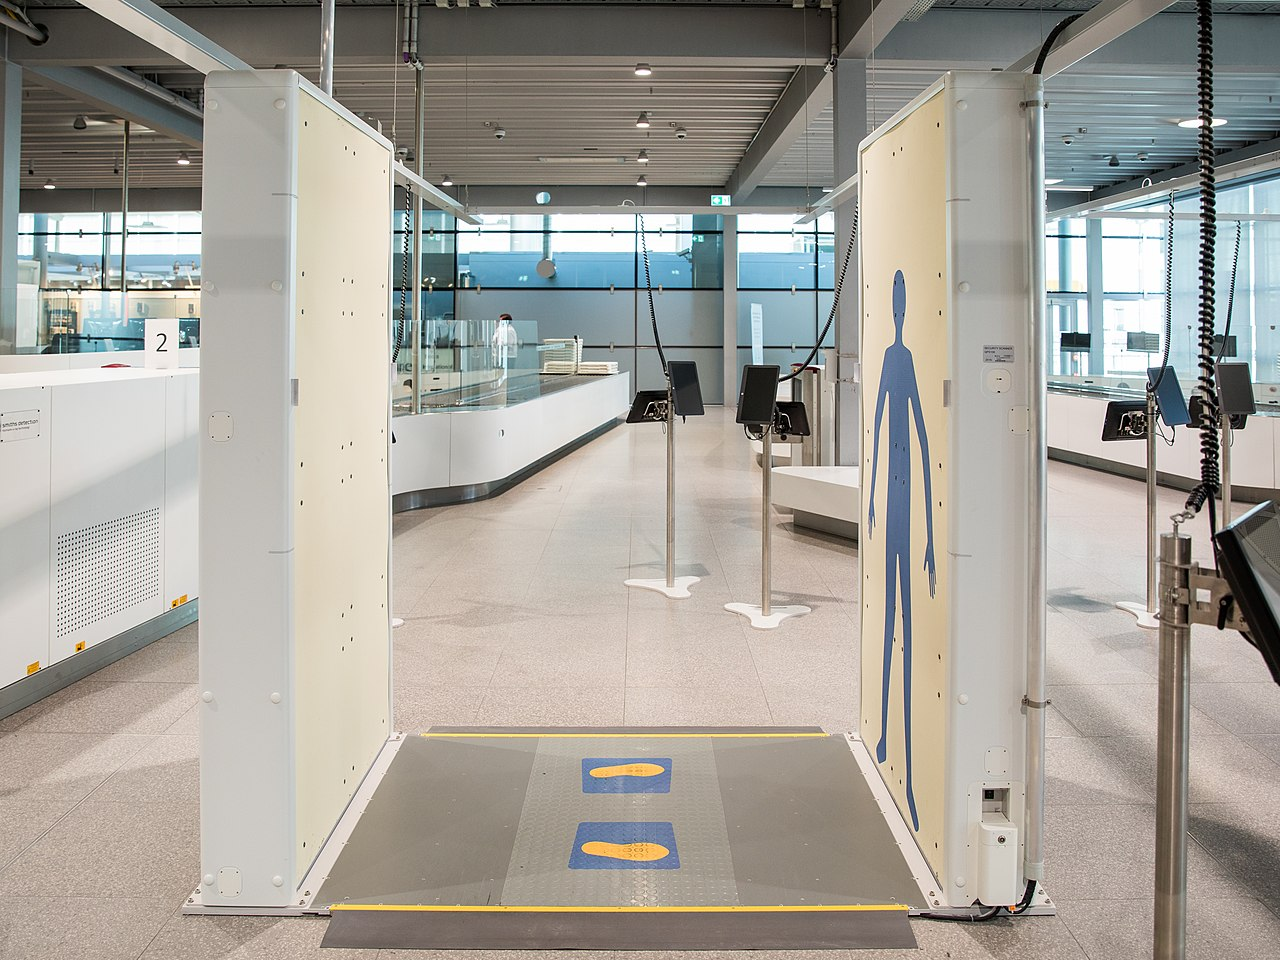
\includegraphics[scale=.12]{mmwavescan.jpg}
        \caption{An airport mm-wave scanner}
        \label{fig:mmwave}
    \end{figure}
    \end{column}
\end{columns}
    
\end{frame}

\begin{frame}{Infrared}
\begin{columns}
    \begin{column}{.5\textwidth}
    Infrared radiation is the part of the spectrum with wavelengths just longer than visible light, and is generally invisible to humans. \vspace{2mm}
    These waves are emitted by anything with thermal energy, and thus can be used to create images based on the temperature of an object. 
    
    \vspace{2mm}
    Because it is invisible to humans, light in the infrared range can also be used for night vision without detection, remote controls, and more. 
    \end{column}
    \begin{column}{.5\textwidth}
    \begin{figure}
        \centering
        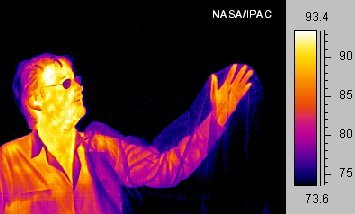
\includegraphics[scale=.35]{infrared1.jpg}
        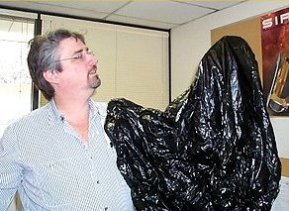
\includegraphics[scale=.35]{infrared2.jpg}
        \caption{Visible light vs thermal imaging}
        \label{fig:infrared}
    \end{figure}
    \end{column}
\end{columns}
\end{frame}

\begin{frame}{Visible Light}
	Visible light is defined as the range that human eyes can percieve, between 400-700nm in wavelength or 430-750 THz. Each wavelength corresponds to a certain color. 
	
	
\includegraphics[scale=.22]{lightspectrum.png}
\end{frame}

\begin{frame}{Sources of Light}
    Most light we care about is emitted by the Sun through black-body radiation simply due to its temperature. Incandescent light bulbs and fire light work the same way, though both emit most light in the infrared. 
    \vspace{2mm}
    
\begin{columns}
    \begin{column}{.5\textwidth}
    Light energy is also released when an atom, electron, or other particle transitions from a high energy state to a lower energy state. The extra energy is released as an EM wave, with wavelength corresponding to the energy released. 
    
    \vspace{2mm}
    
    LEDs, solar panels, and spectroscopy all rely on this.
    
    \end{column}
    \begin{column}{.5\textwidth}
    \begin{figure}
        \centering
        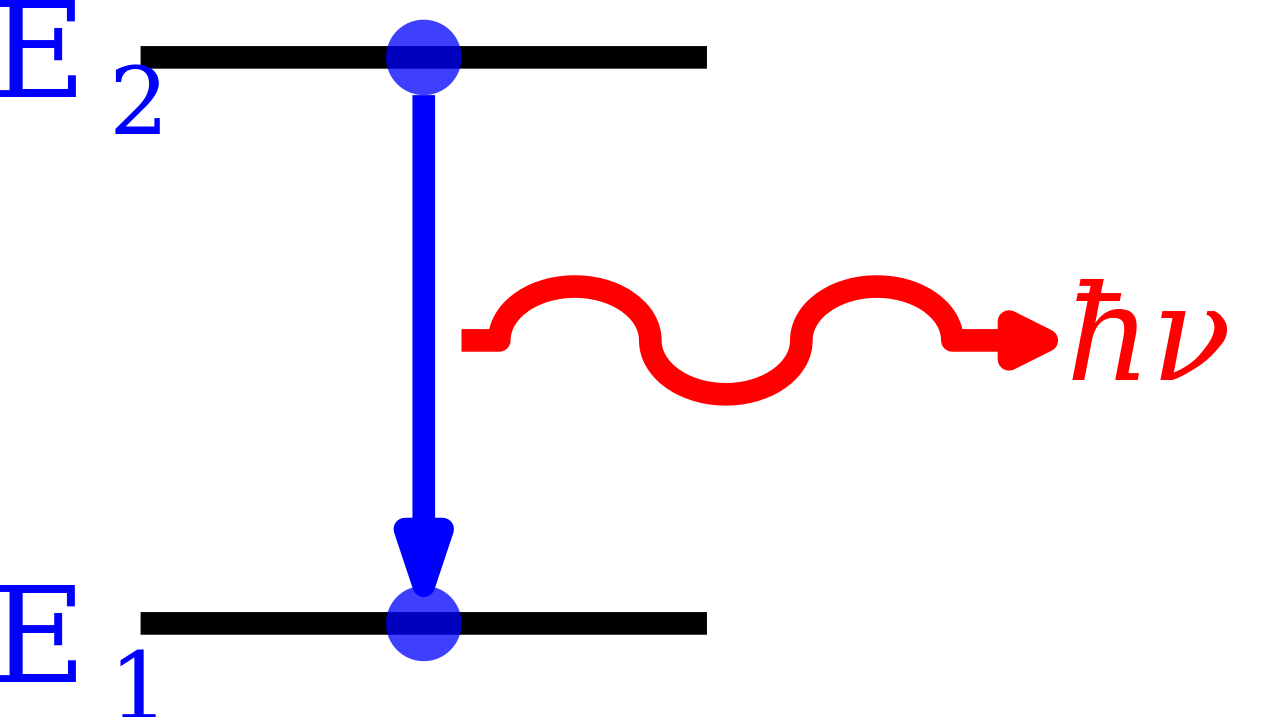
\includegraphics[scale=.1]{emission.png}
        \caption{EM Wave emission due to changing energy levels}
        \label{fig:infrared}
    \end{figure}
    \end{column}
\end{columns}
\end{frame}

\begin{frame}{Atmospheric Phenomenon}
    The same principles, particularly \alert{Raleigh Scattering} is the reason behind the sky's blue color during the day, and the orange-red color of sunrise and sunset. \newline
    
    During the day, the shorter wavelengths of light (blue and green) are \alert{scattered} in the atmosphere, bouncing between particles until it eventually is reflected to earth. \newline
    
    As the sun gets lower, it must pass through more of the atmosphere, so many of these high frequency waves are absorbed completely, leaving only the low frequency waves that diffract better, thus causing red colors. 
\end{frame}

\begin{frame}{Ionizing Radiation}
    The very high frequency EM waves have high enough energy to remove electrons from atoms and molecules, causing ionization. \newline
    
    This ionization can cause damage to cells and DNA, either killing them or causing they to malfunction, leading to increased cancer risk and many other health effects. \newline
    
    Another effect of radiation is temporarily increased electrical conductivity. Electrical current flows through free charges, and ionized atoms have many of these by definition.
\end{frame}

\begin{frame}{X-rays}
X-rays are most famously used for inspecting bones through tissue and for their use in airport security, but they can also be used for determining crystal structure. 

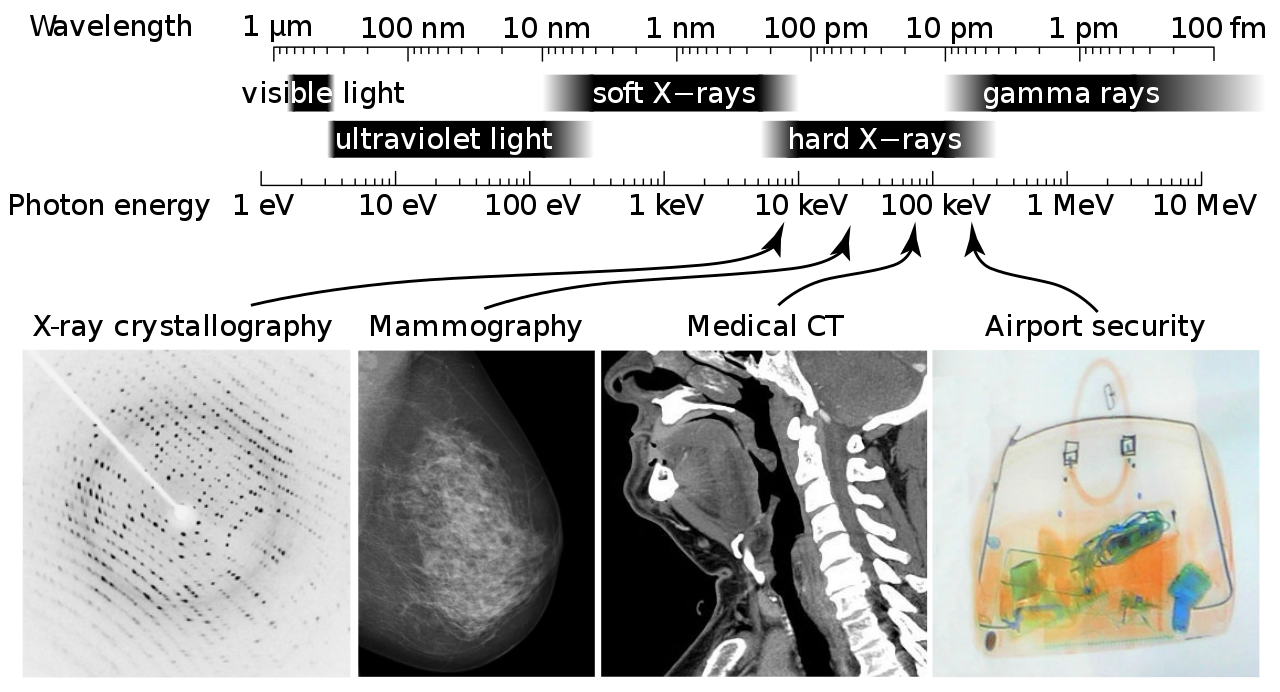
\includegraphics[scale=.25]{xrayuses.png}
\end{frame}

\begin{frame}{Gamma Rays}
    Gamma rays are emitted by the atomic nucleus rather than electrons, and are very dangerous and have a high risk of cancer associated with exposure. Despite this, they have many uses in science and medicine, and are even used to treat cancer.
\end{frame}

\end{document}